% FortySecondsCV LaTeX template
% Copyright © 2019-2020 René Wirnata <rene.wirnata@pandascience.net>
% Licensed under the 3-Clause BSD License. See LICENSE file for details.
%
% Please visit https://github.com/PandaScience/FortySecondsCV for the most
% recent version! For bugs or feature requests, please open a new issue on
% github.
%
% Contributors
% ------------
% * ifokkema
% * Bertbk
% * Hespe
%
% Attributions
% ------------
% * fortysecondscv is based on the twentysecondcv class by Carmine Spagnuolo
%   (cspagnuolo@unisa.it), released under the MIT license and available under
%   https://github.com/spagnuolocarmine/TwentySecondsCurriculumVitae-LaTex
% * further attributions are indicated immediately before corresponding code


%-------------------------------------------------------------------------------
%                             ADDITIONAL PACKAGES
%-------------------------------------------------------------------------------
\documentclass[
	a4paper,
% 	showframes,
% 	vline=2.2em,
    maincolor=myorange,
    sidecolor=myblack,
	sectioncolor=myblue,
	subsectioncolor=mygray!70,
	textcolor=myblue,
%  	itemtextcolor=red
	% sidebarwidth=0.4\paperwidth,
	% topbottommargin=0.03\paperheight,
	% leftrightmargin=20pt,
	profilepicsize=4.5cm,
	profilepicborderwidth=1,5pt,
	profilepicstyle=profilecircle,
	profilepiczoom=1,
	% profilepicxshift=0mm,
	profilepicyshift=-3mm,
	% profilepicrounding=1.0cm,
]{fortysecondscv}

% improve word spacing and hyphenation
\usepackage{microtype}
\usepackage{ragged2e}
% used to set the lenguage
\usepackage[ngerman]{babel}

% uncomment in case you don't want any hyphenation
\usepackage[none]{hyphenat}
\usepackage[hidelinks]{hyperref}

\ifxetexorluatex
	\usepackage{fontspec}
	\usepackage{fontspec,xltxtra} %fonts and styles in xelatex
	\setmainfont{Linux Libertine O}
	\defaultfontfeatures[\rmfamily,\sffamily,\ttfamily]{}
	
% 	\usepackage{raleway}                      % Load raleway font
%     \renewcommand{\familydefault}{\sfdefault} % Set sans serif for document
    %%
	\usepackage{fontawesome}
	% \newfontfamily{\FAFR}{Font Awesome 5 Free Regular}
	% \newfontfamily{\FAFS}{Font Awesome 5 Free Solid}lae
	% \newfontfamily{\FAB}{Font Awesome 5 Brands Regular}
%  	\newfontfamily\headingfont[Path = fonts/]{robot.ttf} % local font
\else
	\usepackage[utf8]{inputenc}
	\usepackage[T1]{robot}
\fi

\usepackage{tikz}
\usetikzlibrary{positioning,fit,calc}
\usetikzlibrary{arrows}


% enable mathematical syntax for some symbols like \varnothing
\usepackage{amssymb}

% bubble diagram configuration
\usepackage{smartdiagram}
\smartdiagramset{
	% default font size is \large, so adjust to harmonize with sidebar layout
	bubble center node font = \footnotesize,
	bubble node font = \footnotesize,
	% default: 4cm/2.5cm; make minimum diameter relative to sidebar size
	bubble center node size = 0.4\sidebartextwidth,
	bubble node size = 0.25\sidebartextwidth,
	distance center/other bubbles = 1.5em,
	% set center bubble color
	bubble center node color = maincolor!70,
	% define the list of colors usable in the diagram
 	set color list = {maincolor!10, maincolor!40,
% 	maincolor!20, maincolor!60, maincolor!35, maincolor!10, maincolor!40,
 	maincolor!20, maincolor!60, maincolor!35, maincolor!5},
% 	% sets the opacity at which the bubbles are shown
	bubble fill opacity = 0.7,
}

%-------------------------------------------------------------------------------
%                            PERSONAL INFORMATION
%-------------------------------------------------------------------------------
%% mandatory information
% your name
\cvname{Giovanni Perez}
% job title/career
\cvjobtitle{DevOps Engineer / \\ System Integrator}

%% optional information
% profile picture
\cvprofilepic{pics/profilegio3.jpeg}

% NOTE: ordering in sidebar will mimic the following order
% date of birth
\cvnation{chilenisch}
\cvbirthday{16.05.1988}
% short address/location, use \newline if more than 1 line is required
\cvaddress{Aretzstr. 52, 52070 Aachen}
% phone number
\cvphone{+49 157 5356 93848}
% personal website
% \cvsite{https://pandascience.net}
% \cvsite{https://gpmontt.github.io/aboutme/}
% email address
\cvmail{giovanni.perez.montt@gmail.com}
\cvring{verheiratet}


%-------------------------------------------------------------------------------
%                              SIDEBAR 1st PAGE
%-------------------------------------------------------------------------------
% add more profile sections to sidebar on first page
\addtofrontsidebar{
	% include gosquare national flags from https://github.com/gosquared/flags;
	% naming according to ISO 3166-1 alpha-2 country codes
	\graphicspath{{pics/flags/}}
	
	\profilesection{Über Mich}
	\aboutme{
    Linux Enthusiast und Hardware-Entwickler. Open Software/Hardware Mentalität. Vim, Tmux und die Konsole sind mein täglich Brot. 
	}

	\profilesection{Sprache}
		\pointskill{\flag{CL.png}}{Spanisch}{4}[4]
		\pointskill{\flag{DE.png}}{Deutsch}{3}[4]
	    \pointskill{\flag{GB.png}}{Englisch}{2}[4]

	% my skill in Software
	\profilesection{Skills}
		\smartdiagram[bubble diagram]{
            \textcolor{black}{{\LARGE \faLinux} \hfil {\Large \faWindows}} \\
			\textcolor{black}{{\Large \faTerminal}}
			\textcolor{black!90}{{\Large \faUbuntu}}, % center bubble,
			{
\includegraphics[width=2em]{pics/cpp_logo.png}}
			{{\Large \faPython} {\Large \faJava}}\\
    		\textcolor{black!90}{{\Large \faMarkdown}}, 
			\textcolor{black!90}{{\large \faDocker} {\Large \faJenkins}},
			\textcolor{black!90}{{\large \faCodeBranch} {\large \faGithub}}\\
			\textcolor{black!90}{{\large \faCode}{\large \faGit} {\large \faGitlab}},
 			\textcolor{black!90}{{\Large \faNetworkWired} {\Large \faServer}}\\
 			{{\Large \faWifi}},
 			%  \textcolor{black!90}{{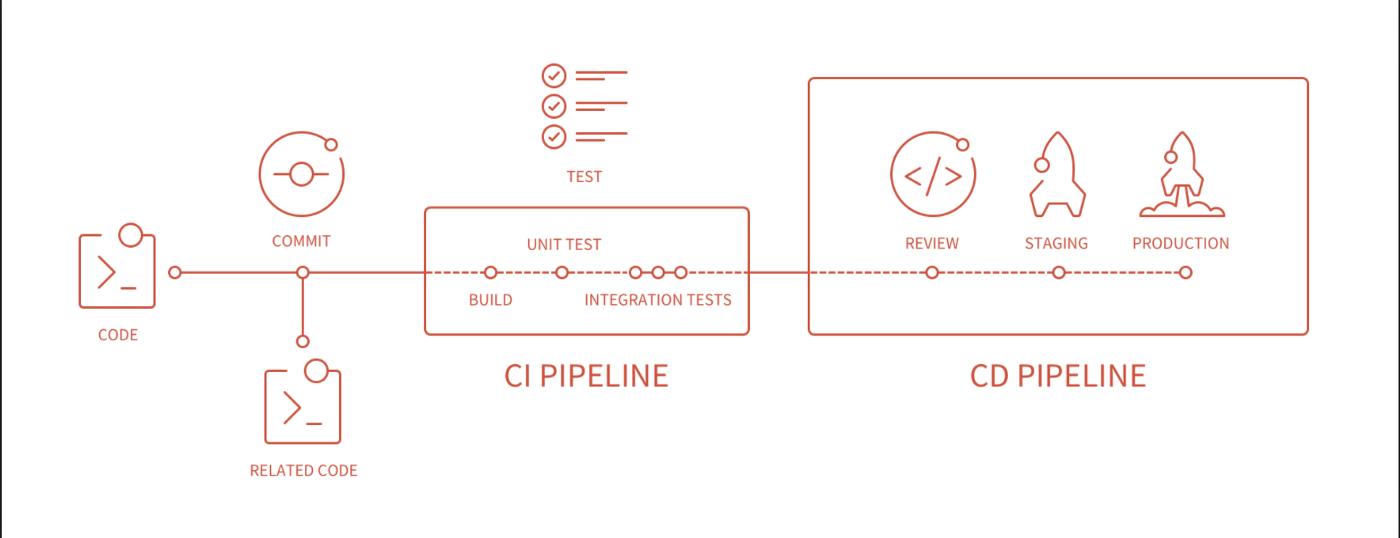
\includegraphics[align=c, width=15em]{pics/cicdgitlab.png}} },
 			{\Large \faLaptopCode} {\Large \faRaspberryPi} 
		 }
	
	
	% 	% social network accounts incl. proper hyperlinks
	\profilesection{Social Network}
		\begin{icontable}{2em}{0.75em}
			\social{\faGithub}
				{https://github.com/gpmontt}
				{@github/gpmontt }
			\social{\faDocker}
				{https://hub.docker.com/u/gpmontt}
				{@docker/gpmontt}	
		\end{icontable}



% 	\profilesection{Hard Skills}
% 		\skill{\faBalanceScale}{Sleeping almost all day}
% 		\skill{\faSitemap}{Eating a lot of bamboo sprouts}
% 		\skill{\faGraduationCap}{Relaxing rest of the day}

% 	\profilesection{Soft Skills}
% 		\pointskill{\faHome}{Looking Cute}{4}[4]
% 			\skill[1.8em]{\faCompress}{No need to specify further}
% 		\pointskill{\faChild}{Chillin' hard}{3}[4]
% 			\skill[1.8em]{\faCompress}{On a tree}
% 			\skill[1.8em]{\faCompress}{In the grass}
}


%-------------------------------------------------------------------------------
%                              SIDEBAR 2nd PAGE
%-------------------------------------------------------------------------------
\addtobacksidebar{

% 	\chartlabel{Wheel Chart}

% 	\wheelchart{3.7em}{2em}{%
% 	25/3em/maincolor!50/Chill,
% 	25/3em/maincolor!15/Play,
% 	25/4em/maincolor!40/Sleep,
% 	25/3em/maincolor!20/Eat
% 	}
% 	\profilesection{About Me}
% 	\aboutme{
% 		The giant panda is a terrestrial animal and primarily spends its life
% 		roaming and feeding in the bamboo forests of the Qinling Mountains and in
% 		the hilly province of Sichuan.
% 		\openmoji \symbol{"1F4D7}
% 	}

% 	\profilesection{Diagrams}
% 	\begin{sidebarminipage}
% 		\chartlabel{Bubble}
% 		\chartlabel{Diagrams}
% 		\chartlabel{with}
% 		\chartlabel{proper}
% 		\chartlabel{overflow}
% 		\chartlabel{protection}
% 		\chartlabel{for}
% 		\chartlabel{labels}
% 	\end{sidebarminipage}

% 	\begin{figure}\centering
% 		\smartdiagram[bubble diagram]{
% 			\textcolor{white}{{\large \faLinux} \hfill {\large \faWindows}}\\
% 			\textcolor{white}{{\large \faMicrochip}}, % center bubble
% 			\textcolor{black!90}{Eating},
% 			\textcolor{black!90}{Sleeping},
% 			\textcolor{black!90}{Rolling},
% 			\textcolor{black!90}{Playing},
% 			\textcolor{black!90}{Chilling}
% 		}
% 	\end{figure}

% 	\chartlabel{Wheel Chart}

% 	\wheelchart{3.7em}{2em}{%
% 	20/3em/maincolor!50/Chill,
% 	15/3em/maincolor!15/Play,
% 	30/4em/maincolor!40/Sleep,
% 	20/3em/maincolor!20/Eat
% 	}

% 	\profilesection{Barskills}
% 	\barskill{\faSkyatlas}{Wearing asian rice hats}{60}
% 	\barskill{\faImage}{Playing Chess}{30}
% 	\barskill{\faMusic}{Playing the bamboo flute}{50}

% 	\profilesection{Memberships}
% 	\begin{memberships}
% 		\membership[4em]{pics/logo.png}{PandaScience.net}
% 		\membership[4em]{pics/logo.png}{Some longer text spanning over more than
% 			only one line}
% 	\end{memberships}
}

%-------------------------------------------------------------------------------
%                         TABLE ENTRIES RIGHT COLUMN
%-------------------------------------------------------------------------------
\begin{document}

\makefrontsidebar
\cvsection{Praktische Erfahrungen {\large \faToolbox}}
\begin{cvtable}[2]
	\cvitem{09/2017--\\bis heute}{Studentische Hilfskraft als \\ Software/Hardware-Entwickler}{Velocitymobility, Aachen}
	{Planung und Implementierung von CI/CD Crosscompiler für Embedded Systems, softwareseitige Pflege des Betriebsystems an den Stationen von Velocity, Entwurf von PCB Platinen für die Integration neuer Module, Einstellungen des Netzwerks für die Stationen, Implementierung eines GPS-Tracking Servers}
	
	\cvitem{09/2017--\\bis heute}{Freelancer \\ Software/Hardware-Entwickler}{3D Punkt LSL UG, Aachen}
	{Verantwortlich für Rapid Prototyping, Entwurf der Elektronik und Software in diversen Industrieprojekten}
	\cvitem{08/2016-- 07/2017}{Wissentschaftliche Hilfskraft}{Maskor Institut, FH-Aachen}
	{Integration von Encoder und GPS IMU für Rover Roboter mit ROS Kinetic}
	\cvitem{09/2015-- 10/2017}{Softwareentwickler}{Indurad GmbH}
	{Verbindung zwischen Servomotor und Steuerungssoftware durch das Protokoll CAN und C++ Umgebung.}
	\cvitem{10/2013-- 03/2014} {Studentische Hilfskraft}{Institut für Kraftfahrzeuge, RWTH Aachen}{Einbindung in Forschungsprojekt:\\
    --Auslegung, Systemaufbau, Inbetriebnahme und Dokumentation für unterschiedliche Schaltanlagen zur Steuerung und Überwachung von Hydraulikanlagen und Elektromotoren von diversen Reifenprüfständen}
	

\end{cvtable}

\cvsection{ Ausbildung {\large \faUniversity}}

\begin{cvtable}[1]
	\cvitem{08/2016-- 03/2020}{Master Elektrotechnik}{FH-Aachen}
		{
		  Student
		}
	\cvitem{06/2014-- 02/2015}{Master Thesis }{„Universidad de Tarapacá“, Chile}
		{
		Künstliches Sehen und Bildverarbeitung für die Entscheidungsfindung eines mobilen Roboters
		}
	\cvitem{07/2012-- 03/2014}{Austauschprogramm des DAAD}{RWTH-Aachen}
		{
        Austauschprogramm des DAAD für ein Jahr an der RWTH Aachen und private Verlängerung Aufenthalt an der RWTH Aachen
		}
	\cvitem{03/2006-- 07/2012}{Studium der Elektrotechnik \\}{„Universidad de Tarapacá“, Chile}
	{ Fachrichtung: Automatisierungstechnik und Robotik 
	}
\end{cvtable}
\cvsection{\textbf{Weiterbildungen}}
\begin{cvtable}[1]
	\cvitem{10/2015-- 01/2016}{Vorbereitung für DSH (Deutsche Sprachprüfung für den Hochschulzugang), Abschlussniveau C1}{Sprachenakademie Aachen}{}
	\cvitem{06/2015}{AUTONAVx: Autonomous Navigation for Flying Robots}{online edX}{}
		
	\cvitem{04/2011-- 08/2012}{CCNA Exploration: LAN Switching and Wireless}{„Universidad de Tarapacá“, Chile}{} 
	\cvitem{08/2010-- 12/2011}{CCNA Exploration: Routing Protocols and Concepts}{„Universidad de Tarapacá“, Chile}{}
	\cvitem{04/2010-- 07/2010}{CCNA Exploration: Network Fundamentals }{„Universidad de Tarapacá“, Chile}{}
\end{cvtable}


\cvsubsection{Dieses Bewerbungsunterlagen wurden mit 'github actions' gebaut\\ (\small{Click auf Icons öffnet Arbeitsschritte zum Nachvollziehen ausgewählter Skills)} }

\centering

\begin{tikzpicture}[->,>=stealth',auto, thick,
  title/.style={align=center},
  typetag/.style={rectangle,rounded corners=2,  draw=black!50}]


%  \draw[help lines,xstep=1,ystep=1]  (-2,0) grid (10,5);

\node[scale=3]                      (github)   at (2,3.1) {\href{https://github.com/gpmontt}{\faGithub}};
\node[align=center,text width=2cm] (githubtitle) [below of=github] {\href{https://github.com/gpmontt}{github/gpmontt}};


\node[text width=3cm,align=center] (user)      at (0,1) {\Large \faUser \faLaptopCode \\\small Local \\Umgebung} ;

\node[fill=gray!20,rectangle,draw,rounded corners=2] (gitact) at (8,4)   {\href{https://github.com/gpmontt/lebenslauf/actions}{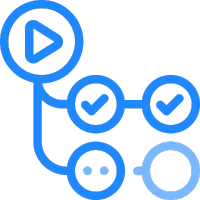
\includegraphics[width=0.05\textwidth]{pics/act.png} {github actions}} 
};

\node[fill=gray!20,rectangle,draw,rounded corners=2,xshift=0.5cm](docker) [below of=gitact] {\href{https://hub.docker.com/r/velocitymob/pandocker}{\Large \faDocker \LaTeX}};

\node[node distance=0.25mm,below= of docker.south]         (checkprocess)   {- check};
\node[node distance=0.25mm,below= of checkprocess.south]   (checkbuild)     {- build};
\node[node distance=0.25mm,below= of checkbuild.south]     (deployprocess)  {- deploy};

\node[fit={(docker) (checkprocess) (checkbuild) (deployprocess) }] (recepy)  {};
\node[draw,rectangle,rounded corners=2 ,fit={(gitact) (recepy)}] (code)  {};

\draw[->, gray!50, very thick] (user) to[out = 90 , in=180 ] node[above,text width=1.5cm,myblue,align=center] {\small modified code\\\LARGE \faFile } (github);
\draw[->, gray!50, very thick] (github) to[out = 0 , in=180 ] node[above,text width=1.5cm,myblue,align=center] {\small clone\\code\\ \LARGE \faCopy} (gitact);
\draw[->, gray!50, very thick] (deployprocess) to[out = 210 , in=270 ] node[above,text width=1.5cm,myblue,align=center] { \href{https://github.com/gpmontt}{\LARGE \faFilePdf\\\small Lebenslauf.pdf}} (githubtitle);

%% reference github actions
\draw[->, myblue, very thick] (gitact) to[out = 0 , in=0 ] node[] {} (docker);
\draw[->, myblue, very thick] (docker) to[out = 180 , in=180 ] node[below] {} (checkprocess);
\draw[->, myblue, very thick] (docker) to[out = 180 , in=180 ] node[below] {} (checkbuild);
\draw[->, myblue, very thick] (docker) to[out = 180 , in=180 ] node[below] {} (deployprocess);


\end{tikzpicture}
\end{document}
